\section{Analyse af kønsforskel}
\label{TestAfSkalaKoensforskel}
%
Det ønskes at undersøge om der er forskel mellem kvinder og mænds besvarelser til skalaerne. Til at undersøge det anvendes Multivariate analysis of variance (MANOVA) som kan betragtes som en ANOVA for situationer hvor der er mere end én afhængig variabel \parencite[s. 697]{FieldMANOVA}. 
De afhængige variable er besvarelserne til skalaerne. Da skalaerne ikke måler det samme, kategoriseres de som forskelle variable, og antallet af afhængige variable vil derfor være det antal af skalaer hvor besvarelserne til ønskes at analyseres. Den uafhængig variabel er kønnet, der består af to grupper, som er henholdsvis mænd og kvinder. 
%
\subsection{Skalabesvarelser der analyseres}
%
Før analysen udføres undersøges det hvilke skalaer der er relevante at analysere i forhold til køn. Ud fra \autoref{fig:BarPlotKoen}, præsenteret i \fullref{TestAfSkalaPraesentationAfData}, bestemmes det er de besvarelser der ser ud til at vareriere i besvarelser mellem mænd og kvinder er SQ 4 \textit{Hvordan oplevede du robottens bevægelser?} (Ekstremt rolige/Ekstremt vilde), SQ11 \textit{Robotten gjorde mig forskrækket }(Helt uenig/Helt enig), SQ13 \textit{Jeg regnede med, at robotten fulgte mig hen til det sted jeg valgte} (Helt uenig/Helt enig) og SQ21 \textit{Hvad synes du ellers om robotten?} (Slet ikke menneskelig/Ekstremt menneskelig). Det vil være disse fire skalabesvarelser der analyseres i følgende afsnit. \blankline
%
\subsection{Testpersoners besvarelser}
%
Analysen udføres i databehandlings programmet R. Dette program kræver, i forhold denne analyse, et fuldstændigt datasæt hvor der ikke mangler nogle værdier. Det er derfor nødvendigt at eksludere besvarelser fra de testpersoner som ikke har besvaret alle fire SQ. De testpersoner hvorfra data eksluderes er testperson 21 og 27 der begge ikke har besvaret SQ 11 og 13. Derudover eksluderes besvarelserne fra testperson 9, 11, 19, 30, 35 og 37 da ingen af dem har besvaret SQ 21. \blankline
%
En oversigt over besvarelserne hvorpå analysen udføres er præsenteret på \autoref{fig:UdvalgteSkalaer}.
%
\begin{figure}[H]
\centering
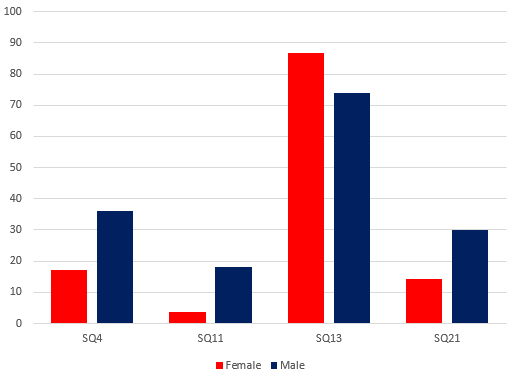
\includegraphics[width = 0.6\textwidth]{Figure/DatabehandlingSkalaer/UdvalgteSkalaerKoen} 
\caption{Søjlediagram over den gennemsnitlige besvarelse til de fire udvalgte skala spørgsmål fordelt på kvinder (rød) og mænd (blå) }
\label{fig:UdvalgteSkalaer}
\end{figure}
\noindent
%
\subsection{Antagelser for MANOVA}
Før MANOVA kan udføres er der fire antagelser der skal opfyldes \parencite[s. 717]{FieldMANOVA}. De fire antagelser minder om dem der er til ANOVA, og er følgende: 

\begin{itemize}
	\item \textbf{Uafhængighed} Observationerne skal være uafhængige af hinanden. 
	\item \textbf{Tilfældig indsamling} Data der analyseres skal være indsamlet tilfældigt fra den ønskede målgruppe og som minimum være målt på en interval skala. 
	\item \textbf{Homogenitet af kovariansmatricer} For hver afhængig variabel skal variansen i hver gruppe være nogenlunde lige. Derudover skal korrelationen mellem hvert par af afhængige variable være den samme i alle grupper. 
	\item \textbf{Multivariat normalitet} At de afhængige variabler har multivariat normalitet indenfor hver gruppe. 
\end{itemize}
%
De første to antagelser der er listet er opfyldt, da dataindsamlingen er baseret på at testpersonerne selv har valgt at interagere med robotten. Observationerne der sammenlignes er afgivet af forskellige personer og derved uafhængige af hinanden. Sidst er besvarelserne afgivet på en VAS skala og opfylder derved antagelsen om at data som minimum skal indsamles på en intervalskala. \blankline
% 
Antagelsen om homogenitet af kovariansmatricerne undersøges ved at opstille varianse-kovarians matricer for hver gruppe, her én for mænd og én for kvinder, for derefter at sammenligne værdierne i matricerne \parencite[s. 725]{FieldMANOVA}. Matricerne for både mænd og kvinder er præsenteret i \autoref{fig:Kovarians}.
%
\begin{figure}[H]
\centering
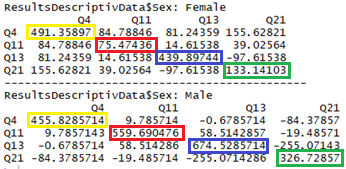
\includegraphics[width = 0.4\textwidth]{Figure/DatabehandlingSkalaer/Normality} 
\caption{Varians-Kovarians matrice for henholdsvis mænd og kvinder. Værdien for SQ4 (gul), SQ11 (rød), SQ13 (blå) og SQ21 (grøn) er markeret i hver matrice.}
\label{fig:Kovarians}
\end{figure}
\noindent
%
For SQ1 er forskellen mellem kønnene ikke så stor (491,456) og det kan derfor konkluderes at SQ1 opfylder antagelsen. For SQ13 (440,675) og SQ21 (133,327) er der lidt større forskel mellem kvinder og mænd, men dog ikke så stor forskel som der kan ses ved SQ11 (75,560). \\
Når der er stor forskel som ved SQ11 undersøges sample størrelserne ift forksellen, for hvis en gruppe har flere målinger end den anden, og det er den største gruppe der har den største varians, vil det være acceptabelt at fortage analysen selvom antagelsen egentlig ikke er opfyldt \parencite[s. 725]{FieldMANOVA}. For de tre SQ hvor der er forskel, er det værdien for gruppen med mænd der er størst og da sample størrelsen for mænd også er større end for kvinderne forsættes analysen. \blankline

For at undersøge antagelsen om multivariat normalitet udføres en Shapiro-Wilk test for multivariate normality \parencite[s. 726]{FieldMANOVA}. \blankline
%
Resultatet af Shapiro normality test er for mænd: W = 0.7303, p-værdi = 6.739e-05 og for kvinder: W = 0.6299, p-værdi = 0.00012. For begge grupper er der signifikant forskel, hvilket betyder at ingen af grupperne har multivariat normalitet og bryder derfor med antagelsen for at udføre MANOVA. \blankline
%
Da antagelsen om multivariat normalitet ikke opfyldes, vælges det at undersøge om det kan skyldes enkelte multivariat outlier, som så kan eksluderes fra analysen \parencite[s. 727]{FieldMANOVA}. På \autoref{fig:AQplot} ses AQ plot for mænd og kvinder.  
%
\begin{figure}[H]
\centering
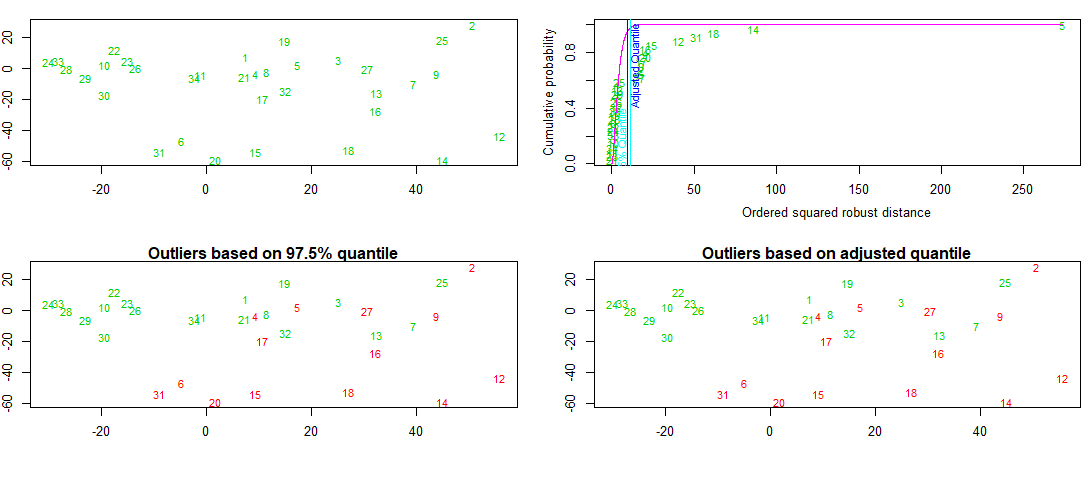
\includegraphics[width = \textwidth]{Figure/DatabehandlingSkalaer/AQplot} 
\caption{AQ plot for køn ift SQ4, SQ11, SQ13 og SQ21.}
\label{fig:AQplot}
\end{figure}
\noindent
%
På AQ plottet er mulige outlier skrevet i rød, og på de nederste to plots kan det ses at besvarelser fra 14 testperson ser ud til at være outlier (2, 4, 5, 6, 9, 12, 14, 15, 16, 17, 18, 20, 27 og 31). \blankline
%
På plottet i øverste højre hjørne på \autoref{fig:AQplot} vil de værdier der ligger til højre for de lodrette linjer (blå og lyseblå) være outlier \parencite[s. 727]{FieldMANOVA}. På dette plottet er der også en del outlier. Da der er del outlier vurderes det at det er for mange datapunkter, til at de kan ekskluderes og forsætte analysen uden dem. Det betyder derfor at antagelsen ikke kan opfyldes, og grundlaget for at udføre en MANOVA på datasættet er der ikke. 
%
\subsection{Robust MANOVA}
%
Ifølge \textcite[s. 733]{FieldMANOVA} er det muligt at udføre en robust MANOVA, som udføres i R ved at anvende pakken \textit{WRS}. Siden bogens udgivelse er denne pakke opdateret til \textit{WRS2} og i denne opdatering er funktionen til udførelse af en robust MANOVA ikke inkluderet. Ifølge \textcite[s. 30]{WEB:WRS2}, der er forfatterne bag pakken, er funktion til robust MANOVA under udvikling, men ikke udgivet endnu. Det er derfor ikke muligt at udføre den robuste MANOVA indenfor tidsrammen af dette projekt. 